\documentclass[11pt]{article}

\usepackage[margin=1.1in]{geometry}
\usepackage{amsmath,amssymb,amsthm}
\usepackage{booktabs}
\usepackage{tikz}
\usepackage{url}
\usepackage[hidelinks]{hyperref}
\usepackage{microtype}

\usetikzlibrary{positioning,arrows.meta}

\emergencystretch=2.5em
\hbadness=10000

\theoremstyle{plain}
\newtheorem{theorem}{Theorem}[section]
\newtheorem{lemma}[theorem]{Lemma}
\newtheorem{corollary}[theorem]{Corollary}
\theoremstyle{definition}
\newtheorem{definition}[theorem]{Definition}

\newcommand{\code}[1]{\texttt{#1}}

\title{Pretrained Language Model Inference on\\ Machine-Checked IEEE-754 Arithmetic}
\author{Charles C. Norton}
\date{September 2026}

\begin{document}
\maketitle

\begin{abstract}
We define the forward pass of three language models in the Rocq prover with all
floating-point arithmetic in IEEE-754 binary32 through Flocq, and extract the
definitions to OCaml. The extracted program loads published \code{safetensors}
checkpoints and performs inference. On GPT-2 (124M parameters),
SmolLM2-135M-Instruct and Qwen3.5-0.8B the extracted forward reproduces the
PyTorch reference's next-token ranking; on the latter two it reproduces the
reference's greedy continuation token for token, and on SmolLM2 its logits to
within $6.1 \times 10^{-5}$ absolute. In the inductive extraction binary32 is Flocq's \code{binary\_float} and
$\mathbb{Z}$ is its inductive datatype, so no floating-point hardware is trusted
anywhere in the forward pass. Eighteen of Qwen3.5's twenty-four layers are gated
DeltaNet blocks, a linear-attention recurrence carrying a per-head state matrix
through the sequence; we give what is to our knowledge the first formalization
of such a recurrence. We prove that cached autoregressive decoding is
bit-identical to full recomputation, for the attention cache and for the
DeltaNet state and convolution window, and identify the two conditions on which
that identity turns: signed zero, and the subnormal mass that masked columns
contribute to the softmax denominator. We give a machine-checked specification
of the \code{safetensors} loader, prove the transposed decode the runners
perform equal to the verified linear layer, and bound each elementary function
against the mathematical function it approximates using CoqInterval. Two defects surfaced. The trigonometric
argument reduction used the magic constant $2^{23}$, which rounds negative
arguments to the nearest half-integer and returns sign-flipped sine and cosine;
and the range-reduced exponential has an irreducible relative error near
$255u \approx 1.5 \times 10^{-5}$, because eight squarings amplify the unit
roundoff by $2^{8}$. Both are diagnosed by computation in Rocq. Repairing the
trigonometric functions, which feed the rotary embedding, improves agreement
with PyTorch by a factor of $65$; repairing the exponential, although it is by
two orders of magnitude the less accurate primitive, changes nothing
measurable. Which primitive matters is not the one its accuracy alone
would suggest.
\end{abstract}

\section{Introduction}

A neural network deployed in float32 has no canonical output. Implementations
disagree across BLAS backends, across fused-multiply-add contraction decisions,
and across GPU reduction orders, and the disagreement is large enough to change
decoded tokens \cite{tinker2025,gensyn2025}. There is consequently no artifact
one can point to and call the answer that a given checkpoint and a given prompt
determine.

The usual route to a formal treatment of a network establishes a property in a
proof assistant and implements the deployed system separately. The deployed
numbers are then a transcription of the proven numbers and the deployed
arithmetic is a separate implementation of the proven arithmetic; in floating
point the two frequently differ. We take the other route. The weights are read,
the arithmetic is performed, and the logits are produced by functions defined in
Rocq and extracted verbatim. No separate implementation is introduced, so the
arithmetic that executes at inference time is the arithmetic the development
reasons about.

The contribution is the conjunction of three properties that are individually
routine and jointly, to our knowledge, unattested: the object is a formal
specification, it is the implementation, and it is validated against the
deployed system on published checkpoints at $10^{8}$ to $10^{9}$ parameters.
Section~\ref{sec:dev} describes the development, Section~\ref{sec:tcb} the two
extraction modes and their trusted bases, and Section~\ref{sec:exec} execution
on pretrained checkpoints. Section~\ref{sec:cache} proves cached decoding
bit-identical to full recomputation. Section~\ref{sec:elem} treats the
elementary functions, where two defects surfaced. Section~\ref{sec:err} treats
the error model, where the existing composed bound is shown unsatisfiable and a
repair is demonstrated. Section~\ref{sec:diff} uses the result as a
differential-testing oracle and Section~\ref{sec:limits} states what remains
unproved.

The development is 14{,}598 lines of Rocq, compiles in under twenty seconds,
and introduces no axioms of its own: \code{Print Assumptions} over the headline
theorems reports exactly four, all of them the classical axioms that
\code{Coq.Reals} introduces and that Flocq's operations inherit, with nine
results closed under the global context.

\section{The development}
\label{sec:dev}

\subsection{Arithmetic}

The floating-point type is Flocq's \code{binary\_float} at precision $24$ and
exponent bound $128$. Addition, multiplication, division, negation, absolute
value, comparison and square root are Flocq's \code{Bplus}, \code{Bmult},
\code{Bdiv}, \code{Bopp}, \code{Babs}, \code{Bcompare} and \code{Bsqrt} at those
parameters under round-to-nearest, ties-to-even. Bit patterns convert both ways
for binary32, binary16 and bfloat16, and the encode/decode round trips are
proved. Decoding a weight from disk goes through Flocq's \code{b32\_of\_bits}
composed with the single-NaN collapse, so a loaded value is the IEEE-754 value
its four bytes denote.

Every scalar the networks compute is produced by one of five primitives:
$+$, $\times$, $\div$, $\sqrt{\ }$ and negation. Everything else is list
plumbing that performs no arithmetic. The elementary functions are compositions
of those five; Section~\ref{sec:elem} treats them in detail.

\subsection{Architectures}

Three families are defined. The GPT-2 path is a pre-norm decoder stack:
layer normalization, fused QKV projection, multi-head causal attention with a
$-10^{9}$ additive mask, residual, layer normalization, GELU feed-forward,
residual, final layer normalization, and a tied-embedding logit projection.
Parameter counts are pinned by reflection; \code{gpt2\_total\_params gpt2\_small}
reduces to $124{,}439{,}808$.

The Llama path replaces layer normalization with RMSNorm, learned position
embeddings with rotary embeddings, multi-head with grouped-query attention, and
the GELU feed-forward with SwiGLU.

The Qwen3.5 path is not a decoder stack. Of its twenty-four layers, eighteen are
gated DeltaNet blocks \cite{gateddeltanet} and six are gated full attention,
alternating with period four. A DeltaNet block projects its input to a fused
query/key/value triple, passes it through a depthwise causal convolution,
$\ell_2$-normalizes query and key, and runs a recurrence over a per-head state
matrix $S \in \mathbb{R}^{d_k \times d_v}$:
\[
  S_t = \operatorname{diag}(e^{g_t})\,S_{t-1}
        + k_t\big(v_t - S_{t-1}^{\top}k_t\big)^{\!\top}\!\beta_t,
  \qquad
  o_t = S_t^{\top} q_t ,
\]
with $g_t = -e^{A_{\log}}\operatorname{softplus}(a_t + b_{\mathrm{dt}})$ and
$\beta_t = \sigma(b_t)$. There is no softmax anywhere in such a block. Writing
$\operatorname{softplus}$ in the stable form
$\max(x,0) + \log(1 + e^{-|x|})$ confines the logarithm to $(1,2]$ and keeps the
function branch-free. The remaining six layers gate their attention output
elementwise by $\sigma$ of a stream carved from the query projection and rotate
only a quarter of each head. For text-only input the interleaved multimodal
rotary embedding collapses to ordinary rotation on that prefix.

\subsection{What is proved}

Serialization round trips for \code{i32} and for the binary32 and binary16 bit
patterns. Storage transformations that invert on every input: chunked split and
reassembly, run-length compression at value, tensor and network level, and
sharding under a byte budget. Dimension preservation through the float stack,
ending in the statements that the forward pass returns one row per input token
and that each logit row has one entry per vocabulary item. Soundness bridges
from boolean checkers to propositions, including a finiteness certificate whose
success entails that every output entry is a finite IEEE-754 value. Prompt
preservation under greedy generation. Correct rounding and a half-ULP accuracy
bound for each of the five primitives, restated at binary32 from Flocq's
correctness lemmas. Harmlessness of the native build's intermediate rounding,
Section~\ref{sec:tcb}. A backward-error statement for the dot product in the
classical form \cite{higham2002}, lifted to the matrix-vector product and to the
tied-embedding projection of all three models. And the results of
Sections~\ref{sec:cache} to \ref{sec:err}. Table~\ref{tab:files} lists the
development by file.

\begin{table}[t]
\centering
\small
\begin{tabular}{llrr}
\toprule
\textbf{File} & \textbf{Content} & \textbf{lines} & \textbf{build} \\
\midrule
\code{Phases1\_15\_complete.v} & definitions, GPT-2, loader, extraction & 5076 & 1.5\,s \\
\code{Float\_error.v}   & rounding, double rounding, composed bounds & 6897 & 6.8\,s \\
\code{Qwen.v}           & gated DeltaNet and gated attention          & 480 & 0.6\,s \\
\code{Llama.v}          & RMSNorm, RoPE, SwiGLU                       & 266 & 0.6\,s \\
\code{Receipt.v}        & inference receipts                          & 87 & 0.6\,s \\
\midrule
\code{Cache.v}          & DeltaNet prefill/decode, convolution window & 257 & 0.7\,s \\
\code{Cache\_attn.v}    & cached attention, transpose involution      & 295 & 0.7\,s \\
\code{Mixed.v}          & mixed error model, vacuity of the old one   & 353 & 0.7\,s \\
\code{Approx.v}         & corrected primitives, CoqInterval bounds    & 231 & 1.5\,s \\
\code{Loader.v}         & loader specification, validation bridge     & 187 & 0.6\,s \\
\code{Runner.v}         & transposed decode equals the linear layer   & 147 & 0.6\,s \\
\code{RoundChk.v}       & the argument-reduction defect, by computation & 80 & 0.6\,s \\
\bottomrule
\end{tabular}
\caption{The development. The upper block predates this paper; the lower block
is its formal contribution. Build times are wall clock under Rocq 9.0.1 with
Flocq on one core, and include roughly $0.55$\,s of process startup each.}
\label{tab:files}
\end{table}

\section{Extraction and the trusted computing base}
\label{sec:tcb}

\begin{figure}[t]
\centering
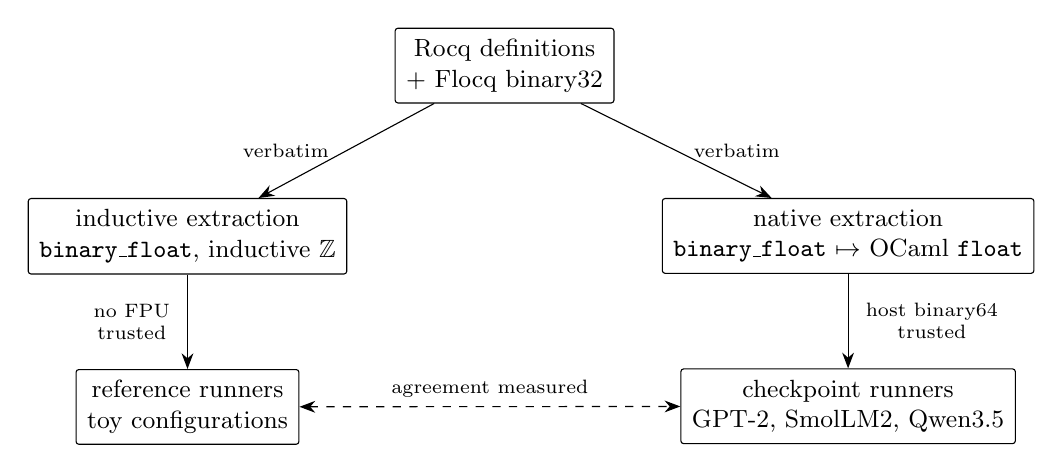
\begin{tikzpicture}[
  node distance=6mm,
  box/.style={draw, rounded corners=1pt, align=center, inner sep=4pt, font=\small},
  lab/.style={font=\scriptsize, align=center},
  >={Stealth[length=2mm]}
]
\node[box] (src) {Rocq definitions\\ + Flocq binary32};
\node[box, below left=12mm and 6mm of src] (ind) {inductive extraction\\ \code{binary\_float}, inductive $\mathbb{Z}$};
\node[box, below right=12mm and 6mm of src] (nat) {native extraction\\ \code{binary\_float} $\mapsto$ OCaml \code{float}};
\node[box, below=12mm of ind] (indr) {reference runners\\ toy configurations};
\node[box, below=12mm of nat] (natr) {checkpoint runners\\ GPT-2, SmolLM2, Qwen3.5};
\draw[->] (src) -- node[lab, left=1mm] {verbatim} (ind);
\draw[->] (src) -- node[lab, right=1mm] {verbatim} (nat);
\draw[->] (ind) -- node[lab, left=1mm] {no FPU\\ trusted} (indr);
\draw[->] (nat) -- node[lab, right=1mm] {host binary64\\ trusted} (natr);
\draw[<->, dashed] (indr) -- node[lab, above] {agreement measured} (natr);
\end{tikzpicture}
\caption{The two extraction modes, emitted from one source by different
directive sets. The inductive mode is the proof artifact; the native mode is the
fast path.}
\label{fig:pipeline}
\end{figure}

The default extraction keeps \code{binary32} as Flocq's inductive
\code{binary\_float} and keeps $\mathbb{Z}$ and \code{positive} as their
inductive datatypes, so every integer operation, and therefore every float
operation built on it, is the computational content of its proof. $\mathbb{Z}$
is not mapped to machine \code{int}: that mapping is unsound when a
mantissa-alignment shift or an intermediate product leaves the representable
range. Only \code{nat}, used for indices, dimensions and token identifiers and
always small, extracts to native \code{int}. This mode introduces no trusted
floating-point boundary at all.

The native extraction maps \code{binary32} to the host's hardware float, in the
manner CompCert extracts its verified floats \cite{compcertfp}. Each operation is
the binary64 result rounded to binary32 through an \code{Int32} bit round-trip.
That the second rounding is harmless is proved by instantiating Flocq's
double-rounding development \cite{roux2014} at the two formats: for operands
representable in binary32, rounding the exact real result of $+$, $-$, $\times$,
$\div$ or $\sqrt{\ }$ to binary64 and then to binary32 equals rounding it
directly to binary32. The width conditions hold because binary64's $53$ bits of
significand exceed binary32's $24$ by the required margin, and the exponent
conditions hold because $e_{\min}^{64} = -1074$ lies far below
$e_{\min}^{32} = -149$.

Sine and cosine are not mapped to the host \code{libm}. They are compositions of
the four arithmetic primitives, so extracting them structurally makes the native
build run the same argument reduction and the same polynomial the inductive
build runs, operation for operation. No library is substituted anywhere in the
forward pass, in either mode. Table~\ref{tab:tcb} states the two trusted bases.

\begin{table}[t]
\centering
\small
\begin{tabular}{lll}
\toprule
& \textbf{Inductive mode} & \textbf{Native mode} \\
\midrule
binary32 values      & Flocq \code{binary\_float}        & OCaml \code{float} \\
$\mathbb{Z}$, \code{positive} & inductive datatypes      & inductive datatypes \\
Arithmetic           & Flocq \code{B}-operations         & host binary64, rounded to binary32 \\
FPU assumed correct  & no                                & yes (binary64, RNE) \\
Elementary functions & five primitives                   & five primitives \\
\code{libm} used     & no                                & no \\
Byte addressing      & native, values via verified decode & native, values via verified decode \\
Extra assumption     & none                              & \code{Int32.bits\_of\_float} rounds to nearest \\
GPT-2 forward pass   & tens of minutes                   & ${\approx}\,7$ s \\
\bottomrule
\end{tabular}
\caption{Trusted computing bases of the two extraction modes. On a small fixture
the two agree bit-identically to nine digits; on GPT-2 they produce identical
token identifiers and logits agreeing to four decimals.}
\label{tab:tcb}
\end{table}

\section{Execution on pretrained checkpoints}
\label{sec:exec}

Applying the definitions to published checkpoints requires addressing two
constraints. The list-based loader cannot ingest a $500$\,MB file, because
representing it as a \code{list byte} builds a linked list of hundreds of
millions of boxed values. And the extracted matrix transpose inside the linear
layer is quadratic in the output dimension through list indexing, which is
acceptable at dimension $8$ and not at $3072$. The checkpoint runners therefore
read file bytes natively, decode each value with the verified
\code{f32\_bytes\_to\_binary32}, and compose the verified primitives in the order
the proven block specifies, decoding each weight matrix already transposed so
that the verified matrix-vector product computes the same dot products the
verified linear layer would. Weights stream layer by layer. That last
substitution is proved correct in Section~\ref{sec:cache}. A $37$-token SmolLM2
forward takes $52.6$\,s and $6.1$\,GB in the native build.

Table~\ref{tab:models} reports the three checkpoints. For GPT-2 on the prompt
\emph{The quick brown}, the extracted greedy next token is $494$, matching the
PyTorch reference, and the top five candidates are returned in the same order.
The logits are offset from the reference's by approximately one unit, because
the feed-forward uses the $x\,\sigma(1.702x)$ form of GELU while GPT-2 was
trained with the tanh form; Section~\ref{sec:elem} quantifies the gap and
supplies the trained form. For SmolLM2 and Qwen3.5 no such substitution occurs
and the extracted logits agree with the reference to within
$6.1 \times 10^{-5}$ absolute and $2.3  imes 10^{-6}$ relative, with identical
top-ten ordering. Section~
ef{sec:elem} accounts for the residual.

\begin{table}[t]
\centering
\small
\begin{tabular}{lccc}
\toprule
& \textbf{GPT-2} & \textbf{SmolLM2-135M-Instruct} & \textbf{Qwen3.5-0.8B} \\
\midrule
Parameters            & 124M            & 135M                  & 0.8B \\
Layers                & 12              & 30                    & 24 \\
Mixer                 & MHA             & grouped-query         & 18 DeltaNet / 6 gated MHA \\
Normalization         & LayerNorm       & RMSNorm               & RMSNorm (zero-centred) \\
Position              & learned         & RoPE                  & partial RoPE \\
Feed-forward          & GELU            & SwiGLU                & SwiGLU \\
Hidden size           & 768             & 576                   & 1024 \\
Vocabulary            & 50\,257         & 49\,152               & 248\,320 \\
\midrule
Argmax matches        & yes             & yes                   & yes \\
Top-$k$ order matches & top 5           & top 8                 & top 8 \\
Logit agreement       & offset ${\approx}1$ & 4 decimals        & 4 decimals \\
Greedy continuation   & ---             & token-identical       & token-identical (8 tokens) \\
\bottomrule
\end{tabular}
\caption{Published checkpoints executed by the extracted forward pass, and
agreement with the PyTorch reference on the chat prompt for
\emph{What is the capital of France?} (GPT-2: \emph{The quick brown}). Qwen3.5
emits $760, 6511, 314, 9338, 369, 2972, 57590, 159034$, byte-identical to the
reference, decoding to \emph{The capital of France is Paris.}}
\label{tab:models}
\end{table}

\section{Cached decoding equals full recomputation}
\label{sec:cache}

Autoregressive generation performs a prefill over the prompt and then one decode
step per token, each reusing state the previous steps produced. The definitions
instead recompute the whole sequence. The two perform the same multiplications
in different groupings, and binary32 addition is not associative, so agreement
is not automatic. It is observed --- Qasim et al.\ decode with and without the
cache on six models spanning 135M to 4B parameters and four architecture
families and report token-identical output in every case \cite{residualstream}
--- but we know of no proof. We give one.

\subsection{The recurrent half}

\code{f32\_delta\_scan} returns the per-token outputs of the gated delta rule and
discards the state. Naming the state as a second recursion, \code{f32\_delta\_state},
describes one pass completely, and the decomposition is exact.

\begin{theorem}[\code{delta\_scan\_app}]
For sequences split anywhere, with the five per-token streams of equal length on
the first part,
\[
  \mathrm{scan}(\beta_1\beta_2, g_1g_2, q_1q_2, k_1k_2, v_1v_2)(S)
  = \mathrm{scan}(\beta_1,\dots)(S)
    \mathbin{+\!\!+} \mathrm{scan}(\beta_2,\dots)\big(\mathrm{state}(\beta_1,\dots)(S)\big).
\]
\end{theorem}

This is an equality of lists of binary32 values, not a bound. Its corollary
\code{delta\_scan\_snoc} is the decode step: extending the sequence by one token
appends exactly the output that step produces from the threaded state and
changes nothing already emitted. \code{delta\_markov} states the consequence
that the outputs after a split depend on the prefix only through the state, which
is what licenses discarding the prompt after prefill.
\code{conv\_window\_cached\_correct} does the same for the depthwise convolution:
the window formed by appending the current input to the trailing $k-1$ entries is
exactly the window \code{f32\_causal\_conv1d} reads, and \code{conv\_hist\_step}
shows the runner's update rule maintains that invariant.

\subsection{The attention half, and two conditions}

\begin{theorem}[\code{attention\_last\_row\_cached}]
Let $q, k$ have $n+1$ rows, let $k$ be rectangular with $c > 0$ columns, and
suppose no attention score of the last row is negative zero. Then attending the
last query over the whole cache equals row $n$ of
\code{f32\_causal\_attention}$(q,k,v,d_k)$, exactly.
\end{theorem}

The proof rests on \code{transpose\_involutive}, that \code{f32\_mat\_transpose}
is involutive on nonempty rectangular matrices, which is closed under the global
context. Two conditions emerged from proving it rather than being assumed.

The first is signed zero. Full attention adds the mask entry to every score, and
on the last row every mask entry is $+0$; the cached path adds nothing. Under
round-to-nearest $x + (+0) = x$ for every binary32 $x$ except $-0$, where it
returns $+0$. We prove both directions: \code{f32\_plus\_zero\_r} for the
identity and \code{f32\_plus\_zero\_neg} for the counterexample. The hypothesis
is therefore exactly the condition under which the two paths coincide, not a
convenience.

The second is that the statement concerns the last row and not earlier ones. On
row $i < n$ the full computation exponentiates the masked columns as well. Those
contribute $e^{-88} \approx 6.05 \times 10^{-39}$, which is subnormal but not
zero, and they enter the softmax denominator; a prefix-cached evaluation omits
them. The two therefore agree only up to whether that subnormal mass survives
rounding, which is not an identity. Decoding computes only the last row, so the
theorem covers the case that runs. The same subnormal reappears in
Section~\ref{sec:err} as the reason the existing composed bound is
unsatisfiable.

\subsection{The transposed decode}

The remaining departure of the runners from the definitions is that they decode
each weight matrix in transposed order rather than calling the quadratic
\code{f32\_mat\_transpose}. \code{decode\_transposed\_correct} proves the decode
returns exactly \code{f32\_mat\_transpose} of the reshape, and
\code{runner\_linear\_correct} concludes that the runner's linear layer computes
the same binary32 values \code{f32\_linear\_forward} computes.

\section{The elementary functions}
\label{sec:elem}

The development's elementary functions are compositions of the five primitives.
\code{Float\_error.v} bounds the float evaluation of each against the \emph{real}
evaluation of the same expression, which says nothing about the distance to the
mathematical function. Supplying that missing half exposed two defects.

\subsection{A defect in the argument reduction}

\code{f32\_round\_int} rounds to the nearest integer by adding and subtracting a
magic constant, and used $2^{23}$. For a non-negative argument the sum lands in
$[2^{23}, 2^{24})$, where the unit in the last place is one, and the result is
the nearest integer. For a negative argument the sum lands in
$[2^{22}, 2^{23})$, where the unit in the last place is one \emph{half}, and the
result is the nearest half-integer: $-0.4$ and $-0.6$ both return $-0.5$. The
reduction then subtracts a half-integer multiple of $2\pi$, shifting the reduced
argument by $\pi$ and flipping the sign of sine and cosine. The absolute error
is $2.0$ on a function bounded by $1$.

\code{RoundChk.v} keeps the superseded definition alongside the one in force and
checks both by computation, so the defect stays checked rather than described.
The constant is now $1.5 \cdot 2^{23} = 12582912$, which keeps the sum in the
correct binade for arguments of either sign. That change alone is
output-neutral on all three models, because rotary angles are
$\mathrm{pos} \times \mathrm{inv\_freq}$ with both factors non-negative, so the
negative branch never executed. The accuracy of the series on non-negative
arguments is a separate matter, and it was not neutral.

\subsection{A structural limit in the exponential}

\code{f32\_exp\_approx} computes $\exp(x/256)^{256}$ by a six-term Taylor series
and eight squarings. Each squaring doubles the incoming relative error, so eight
of them multiply it by $2^{8}$, and the accumulated unit roundoff alone floors
the result near $255u \approx 1.5 \times 10^{-5}$. This is structural: adding
Taylor terms moves the error from $6.46 \times 10^{-5}$ to
$2.71 \times 10^{-5}$ and no further. Replacing the range reduction by
$\exp(x) = 2^{k}\exp(r)$ with $r = x - k\log 2$ removes the amplification
entirely, because scaling by a power of two is exact in binary32. With
Cody--Waite splitting of $\log 2$ and seven Taylor terms, all constants
expressible as quotients of integers that \code{f32\_of\_Z} represents exactly,
the corrected function is more accurate than float32 \code{np.exp}
(Table~\ref{tab:elem}).

\subsection{Which primitive matters}

The exponential is by two orders of magnitude the least accurate primitive in
the development, and the natural expectation is that it dominates the
divergence from the reference implementation. It does not.
Table~\ref{tab:prims} measures each repair on SmolLM2 against PyTorch.
Correcting the exponential changes the agreement by $0.2\%$. Correcting the
trigonometric functions improves it by a factor of $65$, and the two together
by a factor of $121$.

The reason is structural rather than numerical. Sine and cosine are consumed by
the rotary embedding, where their error perturbs the angle of every query and
key in every layer and enters the attention scores directly. The exponential is
consumed by \code{sigmoid} inside SiLU and by \code{softmax}, both of which are
contractions: a relative perturbation of the exponential is damped by the
normalization that follows it. Accuracy of a primitive is therefore not by
itself a guide to its effect, and the development's least accurate function was
not the one worth fixing first.

The corrected reduction and the degree-19 and degree-18 series are now the
definitions in \code{Llama.v}, and \code{Float\_error.v} carries the propagation
relation over them: \code{sin\_reg} and \code{cos\_reg} grew to $67$ and $69$
side conditions and \code{ok\_sin} and \code{ok\_cos} now reach depth $k+20$ and
$k+19$. The corrected exponential is defined and bounded in \code{Approx.v} but
is not the default, because substituting it would rebuild the exponential
machinery of \code{Float\_error.v} for a change Table~\ref{tab:prims} shows to
be immaterial.

\subsection{Bounds against the true functions}

\code{Approx.v} discharges, with CoqInterval, the distance from each polynomial
to the function it approximates, over the interval the reduction guarantees: the
seven-term exponential series within $6 \times 10^{-9}$ of $\exp$, the arctanh
series within $2 \times 10^{-8}$ of $\log$, the degree-19 sine series within
$10^{-9}$ of $\sin$ and the degree-18 cosine series within $10^{-8}$ of $\cos$.
It also proves the superseded eleven-term sine series at least $10^{-4}$ away
from $\sin$ near $\pi$, so the inadequacy is machine-checked rather than
measured. These are statements about real arithmetic; composing them with the
per-operation rounding bounds of \code{Float\_error.v} would give a bound against
the mathematical function, and that composition is not carried out here.

\begin{table}[t]
\centering
\small
\begin{tabular}{lrrr}
\toprule
\textbf{Elementary functions used} & \textbf{max abs} & \textbf{max rel} & \textbf{improvement} \\
\midrule
as published                                  & $3.986\times10^{-3}$ & $1.449\times10^{-4}$ & --- \\
corrected exponential only                    & $3.979\times10^{-3}$ & $1.446\times10^{-4}$ & $1.0\times$ \\
corrected trigonometry only \emph{(in force)} & $6.100\times10^{-5}$ & $2.317\times10^{-6}$ & $65\times$ \\
corrected trigonometry and exponential        & $3.300\times10^{-5}$ & $1.199\times10^{-6}$ & $121\times$ \\
\bottomrule
\end{tabular}
\caption{Divergence of the extracted SmolLM2 forward from the PyTorch reference
over the ten highest-scoring next tokens, under each repair. The top-ten
ordering is identical to PyTorch's in every row. The exponential is the less
accurate primitive by two orders of magnitude and moves the result by $0.2\%$;
the trigonometric functions, which feed the rotary embedding, account for
essentially all of the divergence. The corrected trigonometry costs $66\%$ more
wall clock: a $37$-token forward goes from $31.8$\,s to $52.6$\,s.}
\label{tab:prims}
\end{table}

\begin{table}[t]
\centering
\small
\begin{tabular}{lrrr}
\toprule
& \textbf{development} & \textbf{corrected} & \textbf{float32 library} \\
\midrule
$\exp$, max rel.\ err on $[-88,88]$   & $6.46\times10^{-5}$ & $1.69\times10^{-7}$ & $2.39\times10^{-7}$ \\
$\exp$, max rel.\ err on $[-20,20]$   & $2.68\times10^{-5}$ & --- & $1.93\times10^{-7}$ \\
$\sin$, max abs.\ err, $x \ge 0$, $|x|\le 100$ & $4.50\times10^{-4}$ & $6.5\times10^{-7}$ & $6.0\times10^{-8}$ \\
$\sin$, max abs.\ err on $[-4000,4000]$ & $2.00$ & $6.9\times10^{-7}$ & $6.0\times10^{-8}$ \\
$\log$ on $(1,2]$, max abs.\ err      & $1.02\times10^{-7}$ & --- & --- \\
\bottomrule
\end{tabular}
\caption{Accuracy of the elementary functions against the mathematical
functions. The $2.00$ entry is the sign flip of Section~\ref{sec:elem}: for
negative arguments the current reduction is wrong, not merely imprecise. The
corrected column uses magic constant $1.5\cdot2^{23}$, Cody--Waite splitting of
$\log 2$ and of $2\pi$, and seven and nine series terms respectively. The GELU
substitution costs a further
$\max_x |x\sigma(1.702x) - \mathrm{gelu}_{\tanh}(x)| = 2.07\times10^{-2}$ at
$x = -2.289$, which is the source of the GPT-2 logit offset in
Table~\ref{tab:models}; \code{f32\_gelu\_tanh} supplies the trained form from the
same five primitives.}
\label{tab:elem}
\end{table}

\section{The error model}
\label{sec:err}

\code{Float\_error.v} carries a composed forward bound from the five primitives
through layer normalization, the exponential, softmax, attention, the block and
the stack to the logits. It propagates through the relation \code{regz M z},
which requires $2^{-126} \le |z|$ for every exact intermediate. That is the
condition under which rounding is a pure relative perturbation. It is also false
at zero.

\begin{theorem}[\code{regz\_excludes\_zero}]
For every budget $M$, $\neg\,\code{regz}\ M\ 0$.
\end{theorem}

The forward pass produces exact zeros structurally: the DeltaNet recurrence
starts from an all-zero state matrix, the depthwise convolution zero-pads its
window, and any zero weight or activation zeroes a product inside a dot product.
\code{dotreg\_excludes\_zero\_product} and
\code{f32\_dot\_regular\_excludes\_zero\_product} state the consequence for the
forward and backward premises respectively. Causal masking supplies an
independent obstruction: a masked score shifted by the row maximum is near
$-10^{9}$, the exponential's saturation engages, and the resulting weight is the
subnormal $6.05\times10^{-39}$ of Section~\ref{sec:cache}, which \code{regz}
also rejects. The composed bound is therefore not merely loose; its premises are
unsatisfiable at sequence length two or more, and we do not claim it.

The repair is standard. Flocq's \code{error\_N\_FLT} holds for every real number
with no range hypothesis: rounding is $z(1+d) + e$ with $|d| \le u$,
$|e| \le \eta$ and $de = 0$, so it is relative in the normal range and absolute
near zero. \code{Mixed.v} instantiates this at binary32
(\code{f32\_round\_mixed}), gives the propagation lemmas for addition and
multiplication with no lower bound, and carries the composition through the dot
product: \code{f32\_mac\_step\_mixed} costs one extra $\eta(2+u)$ per
multiply-accumulate against the previous bound, and
\code{f32\_dot\_error\_mixed} accumulates it. The premise is satisfiable where
the old one is not; \code{dot\_ok\_with\_zero} exhibits a dot product one of
whose entries is an exact zero, which \code{dot\_regular\_rejects\_zero} shows
the old relation refuses. The cost is $\eta = 2^{-150}$ per operation against a
bound otherwise measured in multiples of $uM$, so admitting zeros is nearly
free.

This is a demonstration of the repair on the primitives and the dot product.
Rebuilding the whole composition on the mixed model is not done, and with the
pencil-and-paper analysis of transformer inference by Budzinskiy et al.\
\cite{budzinskiy} in the literature, a rebuilt bound would need to improve on it
to be worth stating.

\section{Differential testing}
\label{sec:diff}

Because the extracted forward pass is deterministic and pins every rounding and
every reduction order, it is a fixed reference against which other float32
implementations can be measured. The harness runs a network through the
extracted reference and through a numpy float32 implementation of the identical
elementwise operations with natural numpy reductions, and reports the divergence
and any next-token disagreement. For the Llama and Qwen paths the reference is
the \emph{inductive} extraction, so the oracle trusts no floating-point boundary.
Weights are handed to both sides as raw binary32 bit patterns, so the only
difference is the reduction order.

Divergence tracks width. Moving $d_{\mathrm{model}}$ from $8$ to $64$ at fixed
depth raises the mean absolute logit error by a factor of $19$, while moving
depth from one layer to eight raises it by a factor of $1.6$, and sequence
length and vocabulary size have no discernible effect. That is what accumulating
longer dot products in a different order predicts, and it is consistent with the
probabilistic analysis of rounding-error growth \cite{highammary2019}. The Qwen
rows sit about an order of magnitude above the others, which is what a recurrence
carrying a state matrix across the sequence, on top of a logarithm and a
convolution, predicts.

\begin{table}[t]
\centering
\small
\begin{tabular}{llrrr}
\toprule
\textbf{Path} & \textbf{Configuration} & \textbf{mean abs-err} & \textbf{max abs-err} & \textbf{flips} \\
\midrule
GPT-2  & $L{=}1$, $d{=}8$           & $4.113\times10^{-9}$ & $4.434\times10^{-8}$ & 0/16 \\
GPT-2  & $L{=}2$, $d{=}8$           & $4.489\times10^{-9}$ & $3.021\times10^{-8}$ & 0/16 \\
GPT-2  & $L{=}4$, $d{=}8$           & $5.920\times10^{-9}$ & $1.415\times10^{-7}$ & 0/16 \\
GPT-2  & $L{=}8$, $d{=}8$           & $6.623\times10^{-9}$ & $9.681\times10^{-8}$ & 0/16 \\
GPT-2  & $L{=}4$, $d{=}16$          & $1.233\times10^{-8}$ & $1.267\times10^{-7}$ & 0/16 \\
GPT-2  & $L{=}4$, $d{=}32$          & $3.657\times10^{-8}$ & $3.306\times10^{-7}$ & 0/16 \\
GPT-2  & $L{=}4$, $d{=}64$          & $1.123\times10^{-7}$ & $8.938\times10^{-7}$ & 0/16 \\
GPT-2  & $L{=}4$, $d{=}8$, $T{=}32$ & $4.989\times10^{-9}$ & $4.847\times10^{-8}$ & 0/16 \\
GPT-2  & $L{=}4$, $d{=}8$, $V{=}64$ & $5.570\times10^{-9}$ & $8.566\times10^{-8}$ & 0/16 \\
\midrule
Llama  & $L{=}2$, $d{=}8$           & $6.757\times10^{-9}$ & $5.999\times10^{-8}$ & 0/16 \\
Llama  & $L{=}2$, $d{=}32$          & $4.692\times10^{-8}$ & $3.129\times10^{-7}$ & 0/16 \\
\midrule
Qwen   & $L{=}1$, delta             & $1.049\times10^{-7}$ & $3.741\times10^{-6}$ & 0/16 \\
Qwen   & $L{=}1$, attn              & $1.133\times10^{-7}$ & $3.308\times10^{-6}$ & 0/16 \\
Qwen   & $L{=}4$, delta$^3$/attn    & $3.100\times10^{-7}$ & $5.543\times10^{-6}$ & 0/16 \\
Qwen   & $L{=}2$, $d{=}32$          & $1.074\times10^{-6}$ & $3.248\times10^{-5}$ & 0/16 \\
\bottomrule
\end{tabular}
\caption{Divergence of a numpy float32 mirror from the extracted reference,
selected rows. Sixteen samples per configuration; \emph{flips} counts
final-position next-token disagreements. Across all $23$ configurations and
$368$ samples there are none.}
\label{tab:sweep}
\end{table}

\section{Scope and limitations}
\label{sec:limits}

\paragraph{No equivalence to the reference implementation is proved.}
There is no independently given specification of what GPT-2 computes in
floating point against which the development could be shown correct; the
development is itself such a specification. The agreement with PyTorch reported
in Table~\ref{tab:models} is measured, not proved.

\paragraph{The runners remain partly unverified.}
Section~\ref{sec:cache} closes the two substantive gaps: the cache management
and the transposed decode. The remaining departure is file input and the
structural composition of layers, which is ordinary OCaml and is checked on
fixtures, where the full logit matrix is bit-identical.

\paragraph{The inductive mode has been run at scale only on SmolLM2.}
An inductive \code{binary\_float} carries its mantissa as a chain of
\code{positive} constructors, roughly twenty-five times the footprint of an
OCaml float, so a runner that materialises all 135M parameters at once needs
tens of gigabytes. \code{runners/llama\_talk\_inductive.ml} streams one layer at
a time and holds $2.5$\,GB, at roughly ten minutes per layer against $52.6$\,s
for the whole native forward. GPT-2's inductive runner is the one the repository
already carried; Qwen3.5 has been run inductively only at toy configurations.

\paragraph{One corrected primitive is not the one that runs.}
The repaired argument reduction and the degree-19 and degree-18 trigonometric
series are the definitions in force, and \code{Float\_error.v} carries the
propagation relation over them. The corrected exponential is defined and bounded
in \code{Approx.v} and is not the default: substituting it would rebuild the
exponential machinery of \code{Float\_error.v}, which is built on the structure
of the current definition, for a change Table~\ref{tab:prims} measures at
$0.2\%$. \code{f32\_gelu\_tanh} is likewise available and unused; adopting it
would remove the GPT-2 logit offset at the same cost in the GELU machinery.

\paragraph{The composed forward bound is not claimed.}
Section~\ref{sec:err} shows its premises unsatisfiable and demonstrates the
repair on the primitives and the dot product. The full composition is not
rebuilt.

\paragraph{The receipts do not bind.}
The weight checksum is the rolling hash $\mathrm{acc} \cdot 31 + b \bmod 2^{32}$,
which collides trivially: the byte strings $\langle 01, 00\rangle$ and
$\langle 00, 1\mathrm{F}\rangle$ both hash to $31$. The receipt checker is sound
as stated but binds nothing an adversary could not forge, and we make no claim
for it.

\section{Related work}

Flocq \cite{flocq} provides the IEEE-754 formalization this development computes
in; CompCert's verified floating point \cite{compcertfp} is the model for
extracting Flocq arithmetic to an executable; the double-rounding results
instantiate Roux's development \cite{roux2014}; and Coq's primitive floats
\cite{primfloats} are an alternative route to the same speed with a different
trusted base.

TorchLean \cite{torchlean} is the closest framework-level work: a Lean~4 system
unifying a PyTorch-style API, an executable IEEE-754 binary32 kernel with
explicit trust boundaries, and CROWN/LiRPA-style bound propagation. It
establishes that an executable binary32 semantics in a proof assistant is not
itself new. Its operator set is linear, convolutional and elementwise; it
contains no attention, softmax, state-space or linear-attention primitive, and
its models are trained from random initialization rather than loaded from
published checkpoints. Its end-to-end evaluation covers robustness certificates
for classifiers, physics-informed residual bounds, and a neural controller.
Earlier proof-assistant treatments of neural networks are likewise below the
scale considered here: Certigrad \cite{certigrad} verifies a stochastic
computation graph while modelling reals, MLCert \cite{mlcert} extracts quantized
networks, and Brucker and Stell \cite{brucker} handle feedforward classifiers in
Isabelle/HOL. Jia and Rinard \cite{jiarinard} show that floating-point error in
network verifiers is exploitable, which is the practical case for making the
arithmetic explicit.

For mechanized error analysis the closest work is LAProof \cite{laproof}, which
proves forward and mixed backward bounds for dot products and matrix-vector
products with underflow handled; the mixed model of Section~\ref{sec:err} is
the same device. VCFloat \cite{vcfloat} and its successor treat approximation as
well as rounding error. The dot-product backward-error statement here is the
classical form \cite{higham2002} mechanized at binary32. For transformers
specifically, Budzinskiy et al.\ \cite{budzinskiy} give a mixed-precision
analysis covering LayerNorm against RMSNorm, softmax under attention sinks, and
sequence-length-independent Lipschitz bounds for self-attention.

The determinism problem this development addresses as an oracle is addressed
elsewhere by construction: batch-invariant kernels \cite{tinker2025} and RepOps
\cite{gensyn2025} fix the reduction order in the implementation rather than
specifying it in a proof assistant. Correctly rounded binary32 elementary
functions \cite{rlibm32,coremath} are the alternative to the repaired series of
Section~\ref{sec:elem}; adopting one would make the reference canonical against
mathematics at the cost of moving it further from PyTorch, whose backends are
not correctly rounded. Gated DeltaNet is due to Yang, Kautz and Hatamizadeh
\cite{gateddeltanet}.

\section*{Availability}

The development, the runners, the setup and harness scripts, and the data behind
Tables~\ref{tab:elem} and~\ref{tab:sweep} are at
\url{https://github.com/CharlesCNorton/proof2weights}. It compiles under Rocq~9
with \code{coq-flocq} and, for Section~\ref{sec:elem}, CoqInterval;
\code{theories/Audit.v} reports the assumptions behind the headline theorems.

\begin{thebibliography}{99}

\bibitem{flocq}
S.~Boldo and G.~Melquiond.
\newblock Flocq: A unified library for proving floating-point algorithms in Coq.
\newblock \emph{20th IEEE Symposium on Computer Arithmetic}, 2011.

\bibitem{compcertfp}
S.~Boldo, J.-H.~Jourdan, X.~Leroy, and G.~Melquiond.
\newblock Verified compilation of floating-point computations.
\newblock \emph{Journal of Automated Reasoning}, 54(2):135--163, 2015.

\bibitem{roux2014}
P.~Roux.
\newblock Innocuous double rounding of basic arithmetic operations.
\newblock \emph{Journal of Formalized Reasoning}, 7(1):131--142, 2014.

\bibitem{primfloats}
G.~Bertholon, \'E.~Martin-Dorel, and P.~Roux.
\newblock Primitive floats in Coq.
\newblock \emph{10th International Conference on Interactive Theorem Proving}, 2019.

\bibitem{torchlean}
R.~J.~George, J.~Cruden, W.~Adkisson, X.~Zhong, H.~Zhang, and A.~Anandkumar.
\newblock TorchLean: Formalizing neural networks in Lean.
\newblock arXiv:2602.22631, 2026.

\bibitem{laproof}
A.~Kellison, A.~W.~Appel, M.~Tekriwal, and D.~Bindel.
\newblock LAProof: A library of formal proofs of accuracy and correctness for
  linear algebra programs.
\newblock \emph{30th IEEE Symposium on Computer Arithmetic}, 2023.

\bibitem{vcfloat}
T.~Ramananandro, P.~Mountcastle, B.~Meister, and R.~Lethin.
\newblock A unified Coq framework for verifying C programs with floating-point
  computations.
\newblock \emph{5th ACM SIGPLAN Conference on Certified Programs and Proofs}, 2016.

\bibitem{budzinskiy}
S.~Budzinskiy, W.~Fang, L.~Zeng, and P.~Petersen.
\newblock Numerical stability analysis of large language models.
\newblock arXiv:2503.10251, 2026.

\bibitem{higham2002}
N.~J.~Higham.
\newblock \emph{Accuracy and Stability of Numerical Algorithms}.
\newblock SIAM, second edition, 2002.

\bibitem{highammary2019}
N.~J.~Higham and T.~Mary.
\newblock A new approach to probabilistic rounding error analysis.
\newblock \emph{SIAM Journal on Scientific Computing}, 41(5):A2815--A2835, 2019.

\bibitem{certigrad}
D.~Selsam, P.~Liang, and D.~L.~Dill.
\newblock Developing bug-free machine learning systems with formal mathematics.
\newblock \emph{34th International Conference on Machine Learning}, 2017.

\bibitem{mlcert}
A.~Bagnall and G.~Stewart.
\newblock Certifying the true error: Machine learning in Coq with verified
  generalization guarantees.
\newblock \emph{33rd AAAI Conference on Artificial Intelligence}, 2019.

\bibitem{brucker}
A.~D.~Brucker and A.~Stell.
\newblock Verifying feedforward neural networks for classification in
  Isabelle/HOL.
\newblock \emph{25th International Symposium on Formal Methods}, 2023.

\bibitem{jiarinard}
K.~Jia and M.~Rinard.
\newblock Exploiting verified neural networks via floating point numerical
  error.
\newblock \emph{28th Static Analysis Symposium}, 2021.

\bibitem{gateddeltanet}
S.~Yang, J.~Kautz, and A.~Hatamizadeh.
\newblock Gated Delta Networks: Improving Mamba2 with delta rule.
\newblock \emph{International Conference on Learning Representations}, 2025.

\bibitem{tinker2025}
H.~He and Thinking Machines Lab.
\newblock Defeating nondeterminism in LLM inference.
\newblock September 2025.
\newblock \url{https://thinkingmachines.ai/blog/defeating-nondeterminism-in-llm-inference/}.

\bibitem{gensyn2025}
A.~Arun, A.~St.~Arnaud, A.~Titov, B.~Wilcox, V.~Kolobaric, M.~Brinkmann,
  O.~Ersoy, B.~Fielding, and J.~Bonneau.
\newblock Verde: Verification via refereed delegation for machine learning
  programs.
\newblock arXiv:2502.19405, 2025.

\bibitem{rlibm32}
J.~P.~Lim and S.~Nagarakatte.
\newblock High performance correctly rounded math libraries for 32-bit floating
  point representations.
\newblock \emph{42nd ACM SIGPLAN Conference on Programming Language Design and
  Implementation}, 2021.

\bibitem{coremath}
The CORE-MATH project.
\newblock \url{https://core-math.gitlabpages.inria.fr/}.

\bibitem{residualstream}
K.~U.~Qasim, J.~Zhang, M.~K.~Shaheen, R.~Alharith, and H.~Zhang.
\newblock The residual stream is all you need: On the redundancy of the KV cache
  in transformer inference.
\newblock arXiv:2603.19664, 2026.

\end{thebibliography}

\end{document}
